\section{Boltzmann Machines}
Giriş verileri arasındaki karmaşık ilişkileri modellemek için kullanılır. İsmi, istatistik fizikte Boltzmann dağılımından gelir. Giriş verilerinin özelliklerini öğrenir ve bu özellikler arasındaki ilişkileri modellemek için öğrenilen bir ağırlık matrisi kullanır. İki tür katmana sahiptir:

\begin{figure}[h]
    \centering
    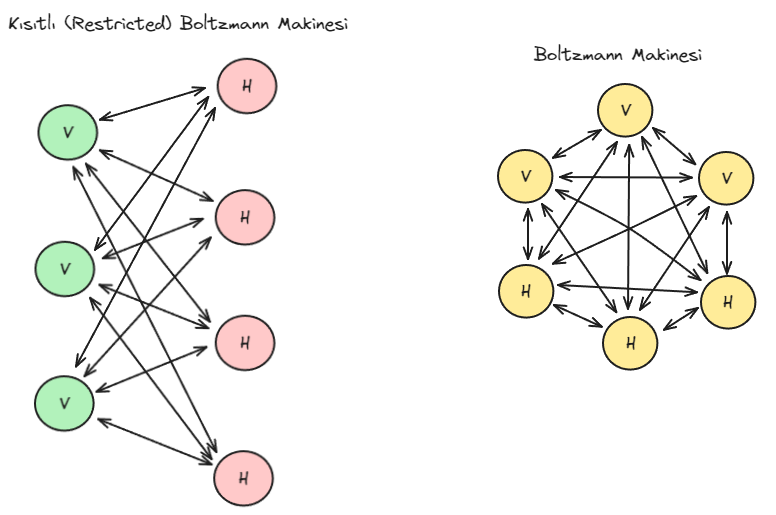
\includegraphics[width=1\textwidth]{images/boltzmann_machines.png}
    \caption{Boltzmann makineleri.}
    \label{fig:enter-label}
\end{figure}

\begin{itemize}
    \item \textbf{Görünür Katman (Visible Layer):} Giriş verilerinin bulunduğu katmandır. Bu katmandaki düğümler, dış dünyadan alınan giriş verilerini temsil eder.
    \item \textbf{Gizli Katman (Hidden Layer):} Görünür katmandaki düğümlerle bağlantılı olan ve karmaşık özellikleri ve ilişkileri temsil eden katmandır. Bu katmandaki düğümler, genellikle giriş verilerinin daha yüksek seviyede özelliklerini temsil eder.
\end{itemize}

"Gibbs Örnekleme" tekniği kullanılarak eğitilir. Bu teknik, rastgele başlangıç değerleriyle başlayarak, modelin öğrenmesi gereken ağırlıkları güncellemek için kullanılır. Gibbs Örnekleme, rastgele başlangıç değerlerine dayalı olarak modele rastgele durumlar üretir ve bu durumlar üzerinde modelin ağırlıklarını günceller.

\subsection{Restricted Boltzmann Machines (RBM)}
Kısıtlı Boltzmann makineleri, tam bağlı katmanlardan farklı olarak kısıtlı bir bağlantı yapısına sahiptir. Bu bağlantı yapısı, gizli ve görünür katmanlar arasındaki tam bağlantıların olmamasıdır. Bu yüzden "kısıtlı" adı verilmiştir. Bu kısıtlama, modelin daha hızlı eğitilmesini ve daha etkili bir şekilde özellikleri öğrenmesini sağlar. İki tür düğüm içerir:
\begin{itemize}
    \item \textbf{Gizli Katman (Hidden Layer):} Görünür katmandaki düğümlerle bağlantılı olan ve modelin özellikleri öğrenmesini sağlayan gizli düğümlerdir.
    \item \textbf{Görünür Katman (Visible Layer):} Giriş verilerinin bulunduğu ve gizli katmandaki düğümlerle bağlantılı olan katmandır.
\end{itemize}

\newpage